% généré depuis source/07_architecture.md — ne pas modifier à la main
\chapter{Architecture et workflow du système}\label{sec:architecture}

\chapintro

Ce chapitre décrit la mise en œuvre logicielle : le pipeline de calcul, l'API, le tableau de bord et les dispositifs qui garantissent la reproductibilité des résultats.

\section{Pipeline de calcul}\label{sec:pipeline}

Le code Python est organisé en modules, un par ticket du plan de sprints (répartition en annexe, \hyperref[sec:annexe-repartition]{«~Annexe D — Répartition du travail~»}). Le script \code{run\_all.py} enchaîne toutes les étapes et exporte les résultats dans des fichiers JSON, qui sont l'unique source de vérité du tableau de bord, des figures, des tableaux et des chiffres de ce rapport :

\begin{verbatim}
data/raw/*.txt
   |  data.py           chargement, RUL, table de durées de vie, description du jeu
   v
fmds.py                 fiabilité, maintenabilité, disponibilité, préventif
features.py             capteurs, features fenêtrées, indicateur de santé
health.py               classification normal / critique
rul_degradation.py      modèle de dégradation bayésien
rul_lstm.py             réseau LSTM
   v
results/  fmds.json  health.json  rul.json  engines.json  dataset.json  run_info.json
   +--> api/main.py (FastAPI)  -->  tableau de bord React
   +--> report_figures.py      -->  report/figures   (PNG et PDF)
   `--> report_tables.py       -->  report/tables, report/generated/valeurs.json
\end{verbatim}

Les modèles entraînés sont sauvegardés dans \code{backend/models/}. Sur la machine de développement, la chaîne complète s'exécute en un peu moins d'une minute lorsque le LSTM de référence est rechargé.

\section{API et endpoints}\label{sec:api}

L'API est développée avec FastAPI (ticket WEB-01, Eya). Elle lit les fichiers JSON, les garde en mémoire et expose cinq routes en lecture :

\begin{itemize}
\item \code{/api/fmds} : indices de fiabilité, de maintenabilité et de disponibilité, et politique préventive ;
\item \code{/api/health} : sélection des capteurs, indicateur de santé et performances des classifieurs ;
\item \code{/api/rul} : métriques, calibration et prédictions des deux modèles de RUL ;
\item \code{/api/fleet} : état actuel des moteurs de test (tableau de flotte) ;
\item \code{/api/engines/\{id\}} : historique complet d'un moteur de test (indicateur de santé, probabilité d'état critique, RUL prédit à chaque cycle).
\end{itemize}

Un identifiant de moteur hors de la plage connue renvoie une erreur \code{404}, un identifiant non numérique une erreur \code{422}, et l'absence des résultats une erreur \code{503} avec un message explicite. La documentation interactive (Swagger) est générée automatiquement. La même application sert le tableau de bord compilé ; elle refuse toute requête qui tenterait de sortir du dossier du tableau de bord.

\section{Tableau de bord}\label{sec:dashboard}

Le tableau de bord (ticket WEB-02, Salma) est une application React avec des graphiques Recharts. Il comporte quatre pages : la vue d'ensemble (figure~\ref{fig:dashboard_overview}), la fiabilité et les indices FMDS (figure~\ref{fig:dashboard_fiab}), le suivi de l'état de santé (figure~\ref{fig:dashboard_mon}) et la durée de vie résiduelle (figure~\ref{fig:dashboard_rul}). Une version \textbf{autonome} en un seul fichier HTML, avec les résultats intégrés, s'ouvre sans serveur ni installation, ce qui facilite la démonstration et la diffusion.

\begin{figure}[htbp]
\centering
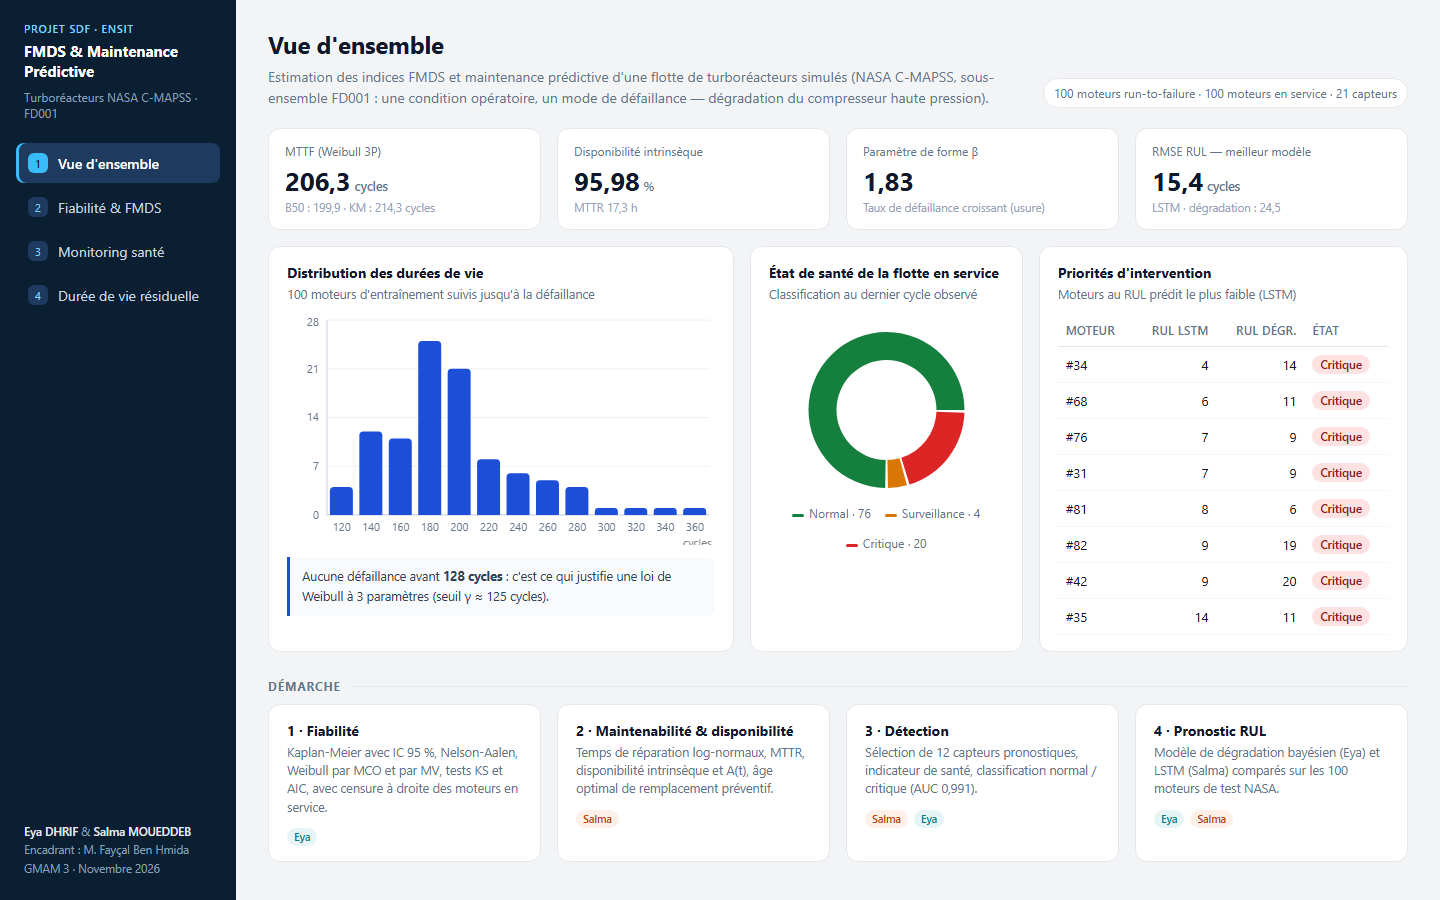
\includegraphics[width=1\linewidth]{figures/dashboard_overview.png}
\caption{Page « Vue d'ensemble » : indicateurs clés, distribution des durées de vie, état de la flotte en service et priorités d'intervention.}\label{fig:dashboard_overview}
\end{figure}

\begin{figure}[htbp]
\centering
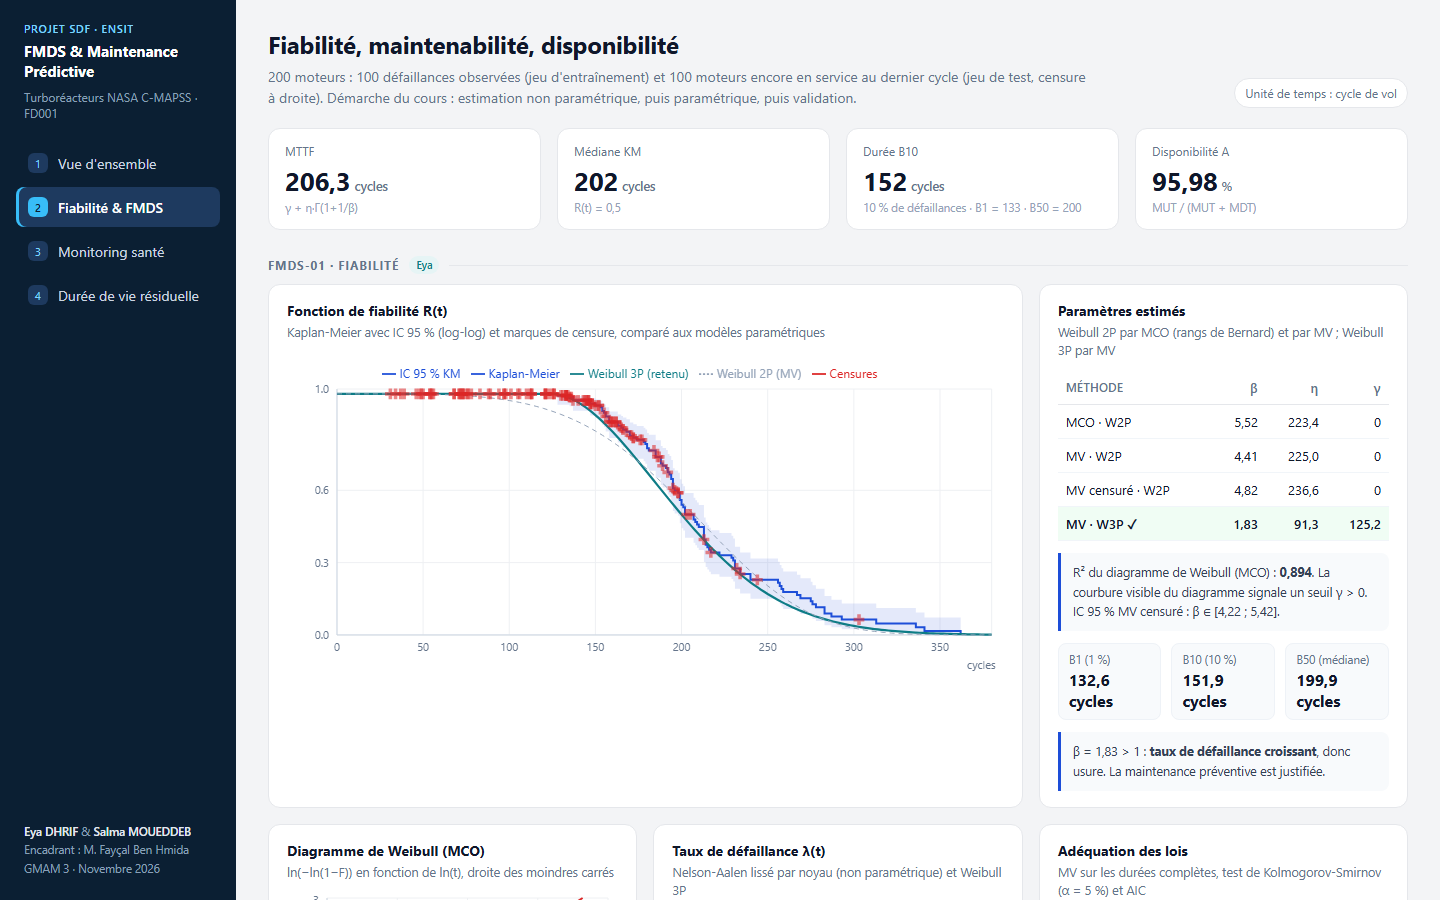
\includegraphics[width=1\linewidth]{figures/dashboard_fiab.png}
\caption{Page « Fiabilité \& FMDS » : fonction de fiabilité, paramètres estimés, adéquation des lois, maintenabilité, disponibilité et politique préventive.}\label{fig:dashboard_fiab}
\end{figure}

\begin{figure}[htbp]
\centering
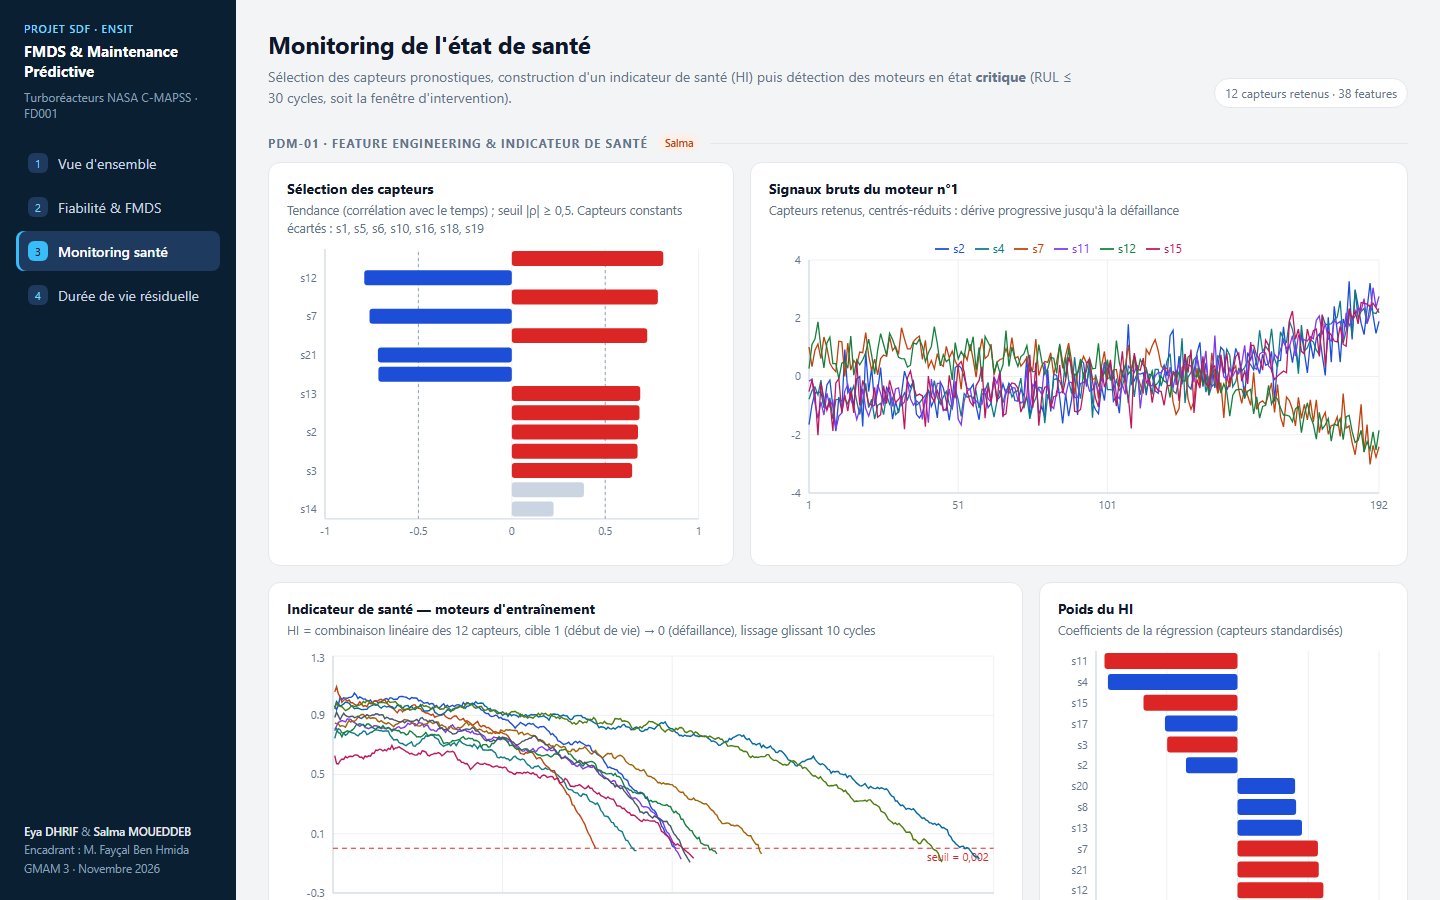
\includegraphics[width=1\linewidth]{figures/dashboard_mon.png}
\caption{Page « Monitoring santé » : sélection des capteurs, indicateur de santé, performances de la classification et suivi d'un moteur.}\label{fig:dashboard_mon}
\end{figure}

\begin{figure}[htbp]
\centering
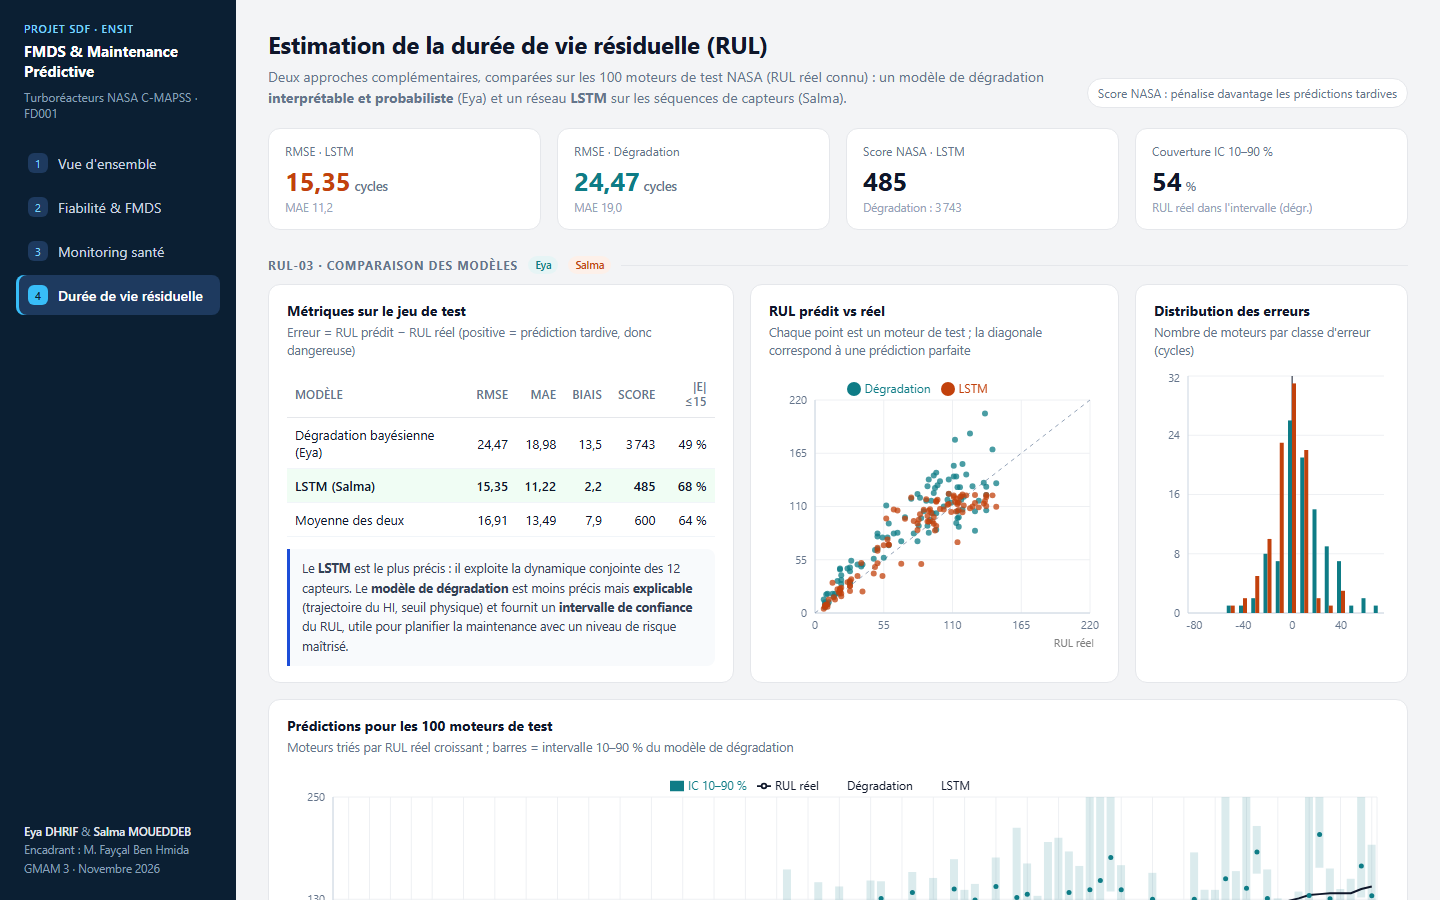
\includegraphics[width=1\linewidth]{figures/dashboard_rul.png}
\caption{Page « Durée de vie résiduelle » : métriques des deux modèles, prédictions pour la flotte, calibration et analyse moteur par moteur.}\label{fig:dashboard_rul}
\end{figure}

\section{Reproductibilité et qualité}\label{sec:reproductibilite}

Plusieurs dispositifs garantissent que chaque chiffre est reproductible et traçable :

\begin{itemize}
\item \textbf{graines fixées} pour toutes les étapes aléatoires (temps de réparation simulés, classifieurs, tirages du modèle de dégradation, LSTM) ;
\item \textbf{modèle LSTM de référence} : un réentraînement sur une autre machine a donné un RMSE légèrement différent, dans la tolérance fixée de plus ou moins un demi-cycle. Les résultats publiés correspondent donc au modèle sauvegardé, que \code{run\_all.py} recharge par défaut ; toutes les autres étapes sont déterministes, et deux exécutions produisent des fichiers JSON identiques. Une installation propre sous Linux redonne les mêmes résultats ; seule une prédiction intermédiaire du LSTM y diffère d'une unité d'arrondi, sans effet sur aucune métrique ;
\item \textbf{traçabilité} : chaque exécution écrit la date, la durée, les versions des bibliothèques et les graines dans \code{run\_info.json}. Les résultats de ce rapport ont été produits avec Python 3.12.10, NumPy 2.5.4, pandas 2.3.3, scikit-learn 1.9.1, lifelines 0.30.3 et PyTorch 2.15.0 ;
\item \textbf{suite de tests automatiques} (pytest pour le calcul et l'API, Playwright pour le tableau de bord). Elle vérifie les méthodes sur des cas dont la réponse est connue, la non-régression de chaque chiffre, l'absence de fuite entre moteurs, la cohérence entre l'API, les fichiers et le tableau de bord, et la concordance de chaque nombre de ce rapport avec sa source.
\end{itemize}

\chapconclusion

Le système repose sur un principe simple : les résultats sont calculés une seule fois par le pipeline, puis servis tels quels à l'API, au tableau de bord et à ce rapport. Le chapitre suivant présente le protocole expérimental et les résultats.
